% NE 630 -- Chapter 4 reading guide, Lessons 15--18
% Standalone source: pdflatex ne630_ch04_reading_guide.tex (twice).
% Layout/palette adapted from the user's ne630boardhandout class.
% Content: supplied chapter(1).tex and lecture_15.tex through lecture_19.tex.
% The supplied chapter numbers the four-factor discussion as Section 4.5.
% Drawings below adapt supplied Fig. 4.1, Fig. 4.5, Fig. 4.6, and the L19
% pin-cell drawing. They are qualitative schematics, not simulation results.
\documentclass[10pt,letterpaper]{article}
\usepackage[T1]{fontenc}
\usepackage[utf8]{inputenc}
\usepackage{libertinus,microtype}
\usepackage[left=0.48in,right=0.48in,top=0.48in,bottom=0.44in,
  headheight=20pt,headsep=5pt,footskip=17pt,includeheadfoot]{geometry}
\usepackage{amsmath,amssymb,mathtools,libertinust1math}
\usepackage{graphicx,xcolor,tabularx,booktabs,array,ragged2e}
\usepackage{tikz}
\usetikzlibrary{arrows.meta,calc,positioning,patterns}
\usepackage[most]{tcolorbox}
\usepackage{fancyhdr,lastpage}
\usepackage[hidelinks]{hyperref}
\hypersetup{pdftitle={NE 630: Chapter 4 Reading Guide -- Lessons 15--18},
 pdfauthor={NE 630},pdfsubject={The Power Reactor Core}}
\definecolor{KSUPurple}{HTML}{512888}
\definecolor{KSUDeepPurple}{HTML}{3B1B64}
\definecolor{KSUOrange}{HTML}{CA7C1B}
\definecolor{KSUGray}{HTML}{5D5D5D}
\setlength{\parindent}{0pt}
\setlength{\parskip}{3pt}
\setlength{\emergencystretch}{1.5em}
\setlength{\abovedisplayskip}{4pt}
\setlength{\belowdisplayskip}{4pt}
\setlength{\abovedisplayshortskip}{2pt}
\setlength{\belowdisplayshortskip}{3pt}
\setlength{\jot}{3pt}
\renewcommand{\arraystretch}{1.12}
\newcolumntype{Y}{>{\RaggedRight\arraybackslash}X}
\newcommand{\LessonNo}{15}
\pagestyle{fancy}
\fancyhf{}
\fancyhead[L]{\sffamily\bfseries\small NE 630}
\fancyhead[C]{\sffamily\small The Power Reactor Core}
\fancyhead[R]{\sffamily\bfseries\small Lesson \LessonNo}
\fancyfoot[L]{\sffamily\scriptsize Chapter 4 \enspace\textbar\enspace Reading guide}
\fancyfoot[C]{\sffamily\scriptsize \thepage\ of \pageref*{LastPage}}
\fancyfoot[R]{\sffamily\scriptsize Read \(\to\) predict \(\to\) test}
\renewcommand{\headrulewidth}{0.5pt}
\makeatletter
\renewcommand{\headrule}{\hbox to\headwidth{\color{KSUPurple}\leaders\hrule height .5pt\hfill}}
\makeatother
\newcommand{\Lesson}[4]{%
  \renewcommand{\LessonNo}{#1}%
  \noindent\begin{minipage}[c]{0.025\linewidth}\color{KSUPurple}\rule{3.5pt}{32pt}\end{minipage}%
  \begin{minipage}[c]{0.815\linewidth}
   {\sffamily\bfseries\fontsize{18}{20}\selectfont #2}\par
   {\sffamily\fontsize{9}{10.5}\selectfont #4}
  \end{minipage}\hfill
  \begin{minipage}[c]{0.14\linewidth}\raggedleft
    {\sffamily\color{KSUPurple}\bfseries\fontsize{25}{26}\selectfont #1}\par
    {\sffamily\scriptsize LESSON}
  \end{minipage}\par\vspace{3pt}
  \begin{tcolorbox}[enhanced,boxrule=.45pt,arc=1pt,colback=KSUPurple!4,
   colframe=KSUPurple!40,left=5pt,right=5pt,top=3pt,bottom=3pt,
   before skip=0pt,after skip=6pt]
   \sffamily\fontsize{9}{10.5}\selectfont\textbf{Read:} #3
  \end{tcolorbox}}
\newcommand{\Sec}[2]{\par\addvspace{5pt}\noindent
  \colorbox{KSUPurple}{\color{white}\sffamily\bfseries\fontsize{9}{10}\selectfont\strut #1}
  \hspace{3pt}{\sffamily\bfseries\color{KSUDeepPurple}\fontsize{10.2}{11.5}\selectfont #2}\par\vspace{1pt}}
\newcommand{\eqread}[1]{{\sffamily\fontsize{7.9}{9}\selectfont\color{KSUGray}#1}}
\newcommand{\figcap}[1]{\par\vspace{1pt}{\sffamily\fontsize{7.7}{9}\selectfont\color{KSUGray}#1}\par}
\newtcolorbox{KeyBox}[1]{enhanced,boxrule=.45pt,arc=1pt,
 colback=KSUPurple!3,colframe=KSUPurple!40,left=5pt,right=5pt,top=4pt,bottom=4pt,
 before skip=4pt,after skip=4pt,before upper=\RaggedRight,fonttitle=\sffamily\bfseries\small,
 coltitle=KSUDeepPurple,title={#1},colbacktitle=KSUPurple!7,
 titlerule=0pt,toptitle=2pt,bottomtitle=2pt}
\newtcolorbox{Explore}[1]{enhanced,boxrule=.5pt,arc=1pt,
 colback=KSUOrange!5,colframe=KSUOrange!65,left=6pt,right=6pt,top=4pt,bottom=4pt,
 before skip=7pt,after skip=3pt,before upper=\RaggedRight,
 title={OpenMC \enspace\textbar\enspace #1},fonttitle=\sffamily\bfseries\fontsize{9}{10}\selectfont,
 coltitle=KSUDeepPurple,colbacktitle=KSUOrange!10,titlerule=0pt,toptitle=2pt,bottomtitle=2pt}
\newcommand{\SourceLine}[1]{\par\vspace{2pt}{\sffamily\fontsize{7.2}{8.4}\selectfont\color{KSUGray}#1}\par}
\newcommand{\colstart}{\begin{minipage}[t]{.482\linewidth}\vspace{0pt}\RaggedRight}
\newcommand{\colnext}{\end{minipage}\hfill\begin{minipage}[t]{.482\linewidth}\vspace{0pt}\RaggedRight}
\newcommand{\colend}{\end{minipage}\par}
\newcommand{\uunit}[1]{\,\mathrm{#1}}
\newcommand{\metal}{\mathrm{metal}}
\newcommand{\water}{\mathrm{w}}
\newcommand{\fiiso}{\mathrm{fi}}
\newcommand{\feiso}{\mathrm{fe}}
\newcommand{\nucl}[2]{\ensuremath{{}^{#1}\mathrm{#2}}}



% Five reactor motifs, adapted from the supplied Fig. 4.1, with a compact TRISO zoom.
\newcommand{\FamilyFigure}{%
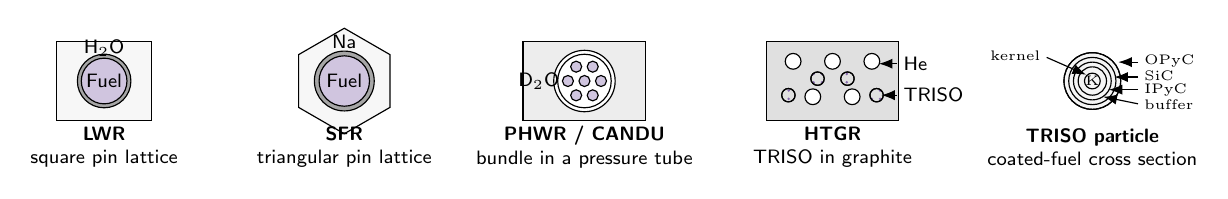
\begin{tikzpicture}[x=1cm,y=1cm,line width=.42pt,font=\sffamily\fontsize{7.5}{8.5}\selectfont,
 every node/.style={inner sep=1pt},>=Latex]
\begin{scope}[shift={(0,0)}]
 \draw[fill=black!3] (-.60,-.50) rectangle (.60,.50);
 \draw[fill=black!35] (0,0) circle (.34);
 \draw[fill=KSUPurple!27] (0,0) circle (.29);
 \node at (0,0) {Fuel}; \node at (0,.42) {H$_2$O};
 \node[align=center] at (0,-.84) {\textbf{LWR}\\square pin lattice};
\end{scope}
\begin{scope}[shift={(3.05,0)}]
 \draw[fill=black!3] (90:.67)--(30:.67)--(-30:.67)--(-90:.67)--(-150:.67)--(150:.67)--cycle;
 \draw[fill=black!35] (0,0) circle (.38);
 \draw[fill=KSUPurple!27] (0,0) circle (.32);
 \node at (0,0) {Fuel}; \node at (0,.50) {Na};
 \node[align=center] at (0,-.84) {\textbf{SFR}\\triangular pin lattice};
\end{scope}
\begin{scope}[shift={(6.10,0)}]
 \draw[fill=black!7] (-.78,-.50) rectangle (.78,.50);
 \draw[fill=white] (0,0) circle (.39);
 \draw (0,0) circle (.34);
 \foreach \ang in {0,60,...,300}{\draw[fill=KSUPurple!27] (\ang:.21) circle (.07);} 
 \draw[fill=KSUPurple!27] (0,0) circle (.07);
 \node[align=center] at (-.58,0) {D$_2$O};
 \node[align=center] at (0,-.84) {\textbf{PHWR / CANDU}\\bundle in a pressure tube};
\end{scope}
\begin{scope}[shift={(9.25,0)}]
 \draw[fill=black!12] (-.84,-.50) rectangle (.84,.50);
 \foreach \x/\y in {-.50/.25,0/.25,.50/.25,-.25/-.20,.25/-.20}{\draw[fill=white] (\x,\y) circle (.10);} 
 \foreach \x/\y in {-.56/-.18,-.19/.03,.19/.03,.56/-.18}{
   \draw[fill=KSUPurple!10,pattern=dots,pattern color=KSUPurple!70] (\x,\y) circle (.085);
   \draw (\x,\y) circle (.085);
 }
 \node[anchor=west] at (.86,.22) {He};
 \draw[->] (.82,.22)--(.59,.22);
 \node[anchor=west] at (.86,-.18) {TRISO};
 \draw[->] (.82,-.18)--(.62,-.18);
 \node[align=center] at (0,-.84) {\textbf{HTGR}\\TRISO in graphite};
\end{scope}
\begin{scope}[shift={(12.55,0)}]
 \draw[fill=KSUPurple!70] (0,0) circle (.10);  % kernel
 \draw[fill=KSUPurple!18] (0,0) circle (.18);  % buffer
 \draw[fill=gray!25] (0,0) circle (.24);       % inner PyC
 \draw[fill=green!12!black!8] (0,0) circle (.30); % SiC
 \draw[fill=gray!8] (0,0) circle (.36);        % outer PyC
 \foreach \r in {.10,.18,.24,.30,.36}{\draw (0,0) circle (\r);} 
 \node[font=\tiny] at (0,0) {K};
 \node[font=\tiny,anchor=west] at (.62,.25) {OPyC}; \draw[->] (.58,.24)--(.33,.24);
 \node[font=\tiny,anchor=west] at (.62,.06) {SiC};  \draw[->] (.58,.05)--(.28,.05);
 \node[font=\tiny,anchor=west] at (.62,-.12) {IPyC};\draw[->] (.58,-.11)--(.21,-.11);
 \node[font=\tiny,anchor=west] at (.62,-.30) {buffer};\draw[->] (.58,-.29)--(.14,-.20);
 \node[font=\tiny,anchor=east] at (-.62,.32) {kernel};\draw[->] (-.58,.30)--(-.08,.08);
 \node[align=center] at (0,-.84) {\textbf{TRISO particle}\\coated-fuel cross section};
\end{scope}
\end{tikzpicture}}

% Square and hexagonal pin cells, adapted from the L19 cell figure and Fig. 4.1.
\newcommand{\PinCellsFigure}{%
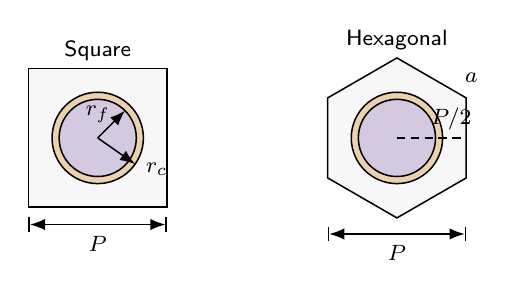
\begin{tikzpicture}[x=1cm,y=1cm,font=\sffamily\fontsize{8.5}{10}\selectfont,
 line width=.55pt,>=Latex,every node/.style={inner sep=1pt}]
\begin{scope}[shift={(0,0)}]
 \draw[fill=black!3] (-.88,-.88) rectangle (.88,.88);
 \draw[fill=KSUOrange!35] (0,0) circle (.58);
 \draw[fill=KSUPurple!25] (0,0) circle (.49);
 \draw[->] (0,0)--(45:.49) node[midway,above left=-1pt] {$r_f$};
 \draw[->] (0,0)--(-35:.58);\node[anchor=west] at (.57,-.40) {$r_c$};
 \draw[|<->|] (-.88,-1.10)--(.88,-1.10) node[midway,below=3pt] {$P$};
 \node at (0,1.10) {Square};
\end{scope}
\begin{scope}[shift={(3.80,0)}]
 \draw[fill=black!3] (90:1.016)--(30:1.016)--(-30:1.016)--(-90:1.016)--(-150:1.016)--(150:1.016)--cycle;
 \draw[fill=KSUOrange!35] (0,0) circle (.58);
 \draw[fill=KSUPurple!25] (0,0) circle (.49);
 \draw[densely dashed] (0,0)--(.88,0);
 \node[above] at (.69,.05) {$P/2$};
 \draw[|<->|] (-.88,-1.22)--(.88,-1.22) node[midway,below=3pt] {$P$};
 \node at (0,1.24) {Hexagonal};
 \node[anchor=west] at (.82,.77) {$a$};
\end{scope}
\end{tikzpicture}}

% Bookkeeping cycle adapted from supplied Fig. 4.5 (not a spatial plot).
\newcommand{\CycleFigure}{%
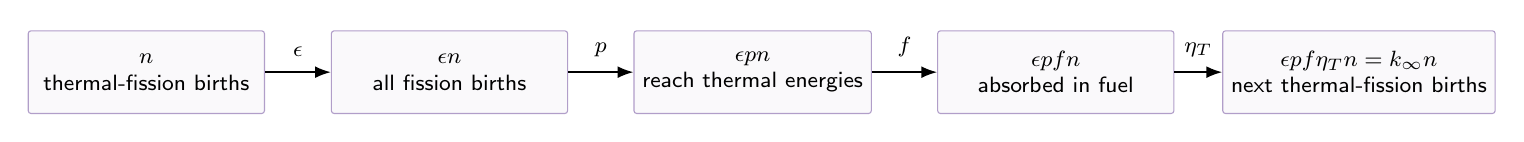
\begin{tikzpicture}[x=1cm,y=1cm,>=Latex,
 box/.style={draw=KSUPurple!45,fill=KSUPurple!3,rounded corners=1pt,
 minimum width=3.0cm,minimum height=1.05cm,align=center,inner sep=3pt},
 every node/.style={font=\sffamily\fontsize{8.2}{9.5}\selectfont}]
 \node[box] (n) at (0,0) {$n$\\thermal-fission births};
 \node[box] (en) at (3.85,0) {$\epsilon n$\\all fission births};
 \node[box] (epn) at (7.7,0) {$\epsilon p n$\\reach thermal energies};
 \node[box] (epfn) at (11.55,0) {$\epsilon p f n$\\absorbed in fuel};
 \node[box] (kn) at (15.4,0) {$\epsilon p f\eta_T n=k_\infty n$\\next thermal-fission births};
 \draw[->,line width=.6pt] (n)--(en) node[midway,above=2pt] {$\epsilon$};
 \draw[->,line width=.6pt] (en)--(epn) node[midway,above=2pt] {$p$};
 \draw[->,line width=.6pt] (epn)--(epfn) node[midway,above=2pt] {$f$};
 \draw[->,line width=.6pt] (epfn)--(kn) node[midway,above=2pt] {$\eta_T$};
\end{tikzpicture}}

% Qualitative Doppler/space-energy shielding sketch, adapted from Fig. 4.6.
\newcommand{\ResonanceFigure}{%
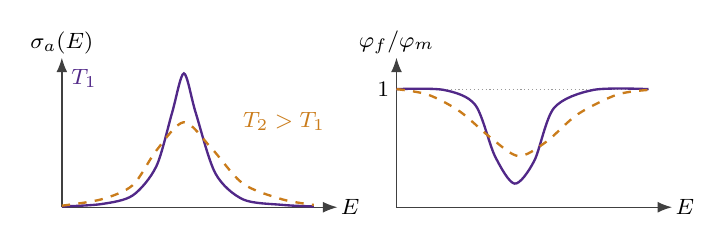
\begin{tikzpicture}[x=1cm,y=1cm,>=Latex,
 ax/.style={->,line width=.5pt,draw=black!75},
 cold/.style={line width=.85pt,draw=KSUPurple},
 hot/.style={line width=.85pt,draw=KSUOrange,dashed},
 every node/.style={font=\sffamily\fontsize{8.1}{9}\selectfont,inner sep=1pt}]
\begin{scope}
 \draw[ax] (0,0)--(3.5,0) node[right] {$E$};
 \draw[ax] (0,0)--(0,1.9) node[above] {$\sigma_a(E)$};
 \draw[cold] plot[smooth] coordinates {(0,.01)(.5,.04)(.9,.15)(1.2,.52)(1.4,1.2)(1.55,1.7)(1.7,1.2)(1.95,.43)(2.3,.10)(2.8,.03)(3.2,.01)};
 \draw[hot] plot[smooth] coordinates {(0,.02)(.5,.10)(.9,.28)(1.2,.72)(1.55,1.08)(1.9,.75)(2.3,.30)(2.8,.10)(3.2,.03)};
 \node[anchor=west,text=KSUPurple] at (.08,1.63) {$T_1$};
 \node[anchor=west,text=KSUOrange] at (2.26,1.09) {$T_2>T_1$};
\end{scope}
\begin{scope}[shift={(4.25,0)}]
 \draw[ax] (0,0)--(3.5,0) node[right] {$E$};
 \draw[ax] (0,0)--(0,1.9) node[above] {$\varphi_f/\varphi_m$};
 \draw[black!40,densely dotted] (0,1.5)--(3.2,1.5);
 \node[anchor=east] at (-.05,1.5) {$1$};
 \draw[cold] plot[smooth] coordinates {(0,1.5)(.6,1.49)(1,1.3)(1.25,.65)(1.5,.3)(1.75,.59)(2,1.26)(2.5,1.49)(3.2,1.5)};
 \draw[hot] plot[smooth] coordinates {(0,1.5)(.4,1.43)(.8,1.22)(1.2,.88)(1.55,.65)(1.9,.83)(2.3,1.18)(2.8,1.43)(3.2,1.49)};
\end{scope}
\end{tikzpicture}}

\begin{document}
\fontsize{9.5}{11.5}\selectfont
\RaggedRight

% ============================ LESSON 15 ============================
\Lesson{15}{From mixtures to reactor lattices}
 {\S\S\,4.1--4.2; Figs.\ 4.1--4.3 and Table 4.1.}
 {Why should moving the same atoms into separate regions change multiplication?}
\begin{center}\resizebox{.97\linewidth}{!}{\FamilyFigure}\end{center}
\vspace{-7pt}
\figcap{Cross-sectional motifs adapted from Fig.\ 4.1, with an added TRISO zoom. Fuel is shaded purple; the stippled HTGR compacts suggest dispersed TRISO particles. These sketches are not on the same scale.}
\colstart
\Sec{1}{Read the core as a coupled design}
Criticality over the fuel lifetime and removal of fission heat jointly determine the lattice. Identify \textbf{fuel, coolant, moderator, cladding/structure, and absorbers}; one material may serve more than one role.
\[
 P_{\rm th}=\bar P'''V,\qquad q'=\frac{P_{\rm pin}}{L},\qquad
 k=k_\infty P_{NL}.
\]
Thin fuel elements shorten heat-conduction distances; assemblies make handling and refuelling practical. A high $k_\infty$ alone does not establish an acceptable power density or a critical finite core.

\begin{tabularx}{\linewidth}{@{}>{\bfseries}p{.67in}Y@{}}
\toprule
Family & Distinction to find in the reading \\
\midrule
PWR/BWR & H$_2$O cools and moderates; enriched UO$_2$. PWR: liquid primary loop and steam generator. BWR: boiling in the core.\\
PHWR & D$_2$O moderator surrounds pressure tubes; low absorption permits natural-U fuel.\\
Graphite & Separate moderator and coolant: He in an HTGR; TRISO particles are embedded in graphite-based fuel compacts or pebbles; boiling H$_2$O in an RBMK.\\
Fast & No intentional moderator; Na (SFR) or He (GCFR) coolant; tightly packed, enriched fuel.\\
\bottomrule
\end{tabularx}

\Sec{2}{Reduce the geometry deliberately}
\textbf{Core $\to$ assembly $\to$ repeating cell.} Use a square or hexagonal cell to represent a uniform lattice. Slabs represent layers, cylinders represent pins, and spheres represent lumps. An equal-volume cylindrical or spherical cell is an \emph{approximation}: preserving volumes does not preserve all neutron paths.
\colnext
\Sec{3}{The uranium-lump experiment}
Begin with H$_2$O and natural U, then segregate U into a central metal sphere of radius $r_U$ inside a water sphere of outer radius $R$. Let $h=H/U$ be the \textbf{total atom ratio}, not a local number-density ratio. With $V_w=V-V_U$,
\[
 h=\frac{N_H^w V_w}{N_U^{\metal}V_U},\qquad
 \boxed{r_U=R\left(\frac{N_H^w}{N_H^w+hN_U^{\metal}}\right)^{1/3}}.
\]
Use nominal $\rho_U=19.1\uunit{g/cm^3}$ for this model and the chosen water density:
\[
 N_U^{\metal}=\frac{\rho_U N_A}{\overline M_U},\qquad
 N_H^w=\frac{2\rho_wN_A}{M_{\mathrm{H_2O}}}.
\]
Here $N_A$ is Avogadro's constant and $M$ denotes molar mass. For the homogeneous comparator, distribute the \emph{same isotope inventories} over $V$:
\[
 \overline N_i=\frac{N_i^{\metal}V_U+N_i^wV_w}{V}.
\]
\textbf{Same $H/U$ alone is not sufficient}: also match the total atoms, outer volume, temperatures, nuclear data, and boundary treatment.

\begin{KeyBox}{The ``a ha'' to look for}
Most slowing down can occur outside the fuel. Near U-238 capture resonances, absorption depresses the flux inside a lump, shielding its interior. This can improve resonance escape without adding fissile atoms. Thermal-flux depression competes with that benefit; larger lumps are not unconditionally better.
\end{KeyBox}
Lumping does \emph{not} by itself make natural uranium in light water critical. Revisit that limitation when $p$ and $f$ are separated in Lessons 17--18.
\colend
\begin{Explore}{Hold the atoms fixed; change their arrangement}
Compare homogeneous and lumped eigenvalue models over $H/U$. Inspect $k$, fuel/water spectra, and U-238 capture. First use the same no-leakage idealization in both models; a reflecting sphere is not an exact lattice tiling. Then add a vacuum boundary to expose leakage. \textbf{Explain:} which energy range accounts for the change in multiplication?
\end{Explore}
\SourceLine{Sources: supplied Ch.\ 4, \S\S\,4.1--4.2 and the self-shielding discussion in \S\,4.5; slide set 15. OpenMC reference: \href{https://docs.openmc.org/en/stable/usersguide/geometry.html}{Geometry, \S\,6.1.1 (boundary conditions)}.}

\newpage
% ============================ LESSON 16 ============================
\Lesson{16}{Fast-reactor unit cells}
 {\S\,4.3, Eqs.\ (4.1)--(4.16); revisit the fast-reactor discussion in \S\,4.2.}
 {When is volume mixing a good approximation to a heterogeneous lattice?}
\colstart
\Sec{1}{Hexagonal arithmetic before transport}
$P$ is nearest-neighbor pin pitch, $D=2r_f$ is \emph{fuel} diameter, $r_c$ is outer cladding radius, and $L$ is a common axial length. A triangular array of pin centers has a hexagonal cell:
\[
 a=\frac{P}{\sqrt3},\quad \text{apothem}=\frac P2,\quad
 A_{\rm hex}=\frac{\sqrt3}{2}P^2,\quad A_{\rm sq}=P^2.
\]
\begin{center}\resizebox{.74\linewidth}{!}{\PinCellsFigure}\end{center}
\vspace{-6pt}
\figcap{Same pitch and pin size, different cell areas. The hexagon's side $a$ is not its across-flats dimension $P$.}
Omitting the gap and assigning the cladding to $st$,
\begin{align*}
 V_f&=\pi r_f^2L, & V_{st}&=\pi(r_c^2-r_f^2)L,\\
 V_c&=(A_{\rm cell}-\pi r_c^2)L, & V&=A_{\rm cell}L.
\end{align*}
Thus, for the hexagonal cell,
\[
 \frac{V_f}{V}=\frac{\pi}{2\sqrt3}\left(\frac DP\right)^2,
 \qquad P>2r_c
\]
for a nonzero inter-pin coolant gap. Extra structure or a fuel--clad gap must be counted separately.

\Sec{2}{Compare length scales, not just energies}
Mean free path and optical thickness:
\[
 \lambda_y(E)=\frac1{\Sigma_t^y(E)},\qquad
 \tau_y(E)=d_y\Sigma_t^y(E).
\]
Fast-energy cross sections are often small. For $d_y\ll\lambda_y$, spatial flux differences are modest:
\[
 \varphi_f(E)\simeq\varphi_c(E)\simeq\varphi_{st}(E).
\]
Test this approximation, especially near resonances. A fast spectrum is not monoenergetic: scattering and absorption still reshape the fission-source spectrum.
\colnext
\Sec{3}{Collapse only after finding the spectrum}
For a common spectrum $\varphi(E)$, define
\[
 \phi=\int_0^\infty\varphi(E)\,dE,\qquad
 \overline\Sigma_x^y=\frac{\int_0^\infty\Sigma_x^y(E)\varphi(E)\,dE}{\phi}.
\]
Volume mixing then gives $\Sigma_x=\sum_y(V_y/V)\Sigma_x^y$. The chapter's production/absorption balance becomes
\[
 \boxed{k_\infty\simeq
 \frac{V_f\overline{\nu\Sigma_f}^{\,f}}
 {V_f\overline\Sigma_a^f+V_c\overline\Sigma_a^c+V_{st}\overline\Sigma_a^{st}}.}
\]
\eqread{Eqs.\ (4.2)--(4.8); leakage and nonfission neutron multiplication neglected.}

Average $\nu\Sigma_f$ as a \emph{product}, not as $\bar\nu\,\overline\Sigma_f$.

\Sec{4}{Enrichment is the fast-lattice lever}
In the two-nuclide model ($fi$: fissile; $fe$: fertile),
\[
 N_f=N_{fi}+N_{fe},\qquad \widetilde e=\frac{N_{fi}}{N_f}.
\]
Let $a_i=\overline\sigma_a^{\,i}$, $b_i=\overline{\nu\sigma_f}^{\,i}$ and
\[
 C=\frac{V_c\overline\Sigma_a^c+V_{st}\overline\Sigma_a^{st}}{V_fN_f}.
\]
At a \emph{fixed spectrum}, Eq.\ (4.16) is
\[
 k_\infty(\widetilde e)=
 \frac{b_{fe}+\widetilde e(b_{fi}-b_{fe})}
 {a_{fe}+\widetilde e(a_{fi}-a_{fe})+C}.
\]
Solving for an assigned lattice target $k_*$ gives
\[
 \widetilde e_*=
 \frac{k_*(a_{fe}+C)-b_{fe}}
 {(b_{fi}-b_{fe})-k_*(a_{fi}-a_{fe})}.
\]
Retest this fixed-spectrum estimate after composition changes. Finite cores also need leakage and fuel-life margins.

\textbf{Match the enrichment basis:} $\widetilde e$ is an atom fraction; OpenMC's uranium \texttt{add\_element} uses U-235 \emph{weight percent}. Convert, or set isotope atom fractions explicitly.
\colend
\begin{Explore}{Test homogenization; then vary SFR enrichment}
Compare a fuel--cladding--Na hexagonal cell with its inventory-matched homogeneous mixture. Set \texttt{HexagonalPrism}'s \texttt{edge\_length} to $P/\sqrt3$. Suppress axial and lateral leakage; compare regional spectra, $k_\infty$, and absorption shares. Sweep enrichment and test the fixed-spectrum estimate against transport. \textbf{Explain:} why does extra coolant change both parasitic absorption and the collapsed fuel data?
\end{Explore}
\SourceLine{Sources: Ch.\ 4, \S\,4.3; slide sets 16--17. OpenMC: \href{https://docs.openmc.org/en/stable/pythonapi/generated/openmc.model.HexagonalPrism.html}{HexagonalPrism}; \href{https://docs.openmc.org/en/stable/pythonapi/generated/openmc.Material.html}{Material.add\_element}.}

\newpage
% ============================ LESSON 17 ============================
\Lesson{17}{Thermal cells and the four factors}
 {\S\,4.4 and the four-factor development in \S\,4.5; Eqs.\ (4.17)--(4.28), (4.42)--(4.51).}
 {Which part of the neutron life cycle explains a change in multiplication?}
\begin{center}\resizebox{.995\linewidth}{!}{\CycleFigure}\end{center}
\vspace{-7pt}
\figcap{Idealized no-leakage cycle (adapted from Fig.\ 4.5). Thermal fission produces \emph{fast} neutrons. The four factors describe coupled processes.}
\colstart
\Sec{1}{Keep space and energy together}
At thermal and resonance energies, larger optical thicknesses produce substantial fuel/moderator flux differences. Use \textbf{regional volume averages} $\varphi_y(E)$; the flux need not actually be uniform inside a homogeneous material region.

\textbf{Bands:} $T$: $E<1\uunit{eV}$; $I$: $1\uunit{eV}\le E<0.1\uunit{MeV}$; $F$: $E\ge0.1\uunit{MeV}$. ``Nonthermal'' means $I\cup F$, not just $F$.

For band $g$ and region $y$, introduce volume-integrated absorption and fission-neutron production:
\begin{align*}
 A_g^y&=V_y\int_g\Sigma_a^y(E)\varphi_y(E)\,dE,\\
 B_g^y&=V_y\int_g\nu\Sigma_f^y(E)\varphi_y(E)\,dE.
\end{align*}
Only fuel fissions: $B_g=B_g^f$, $B=\sum_g B_g$, and $A=\sum_{g,y}A_g^y$. With $A_T=A_T^f+A_T^m$, the chapter's two-region model retains
\[
 B\simeq B_T+B_F,\qquad A\simeq A_T+A_I^f,
\]
and hence $k_\infty\simeq(B_T+B_F)/(A_T+A_I^f)$.
\eqread{Eqs.\ (4.18)--(4.23): intermediate fission, fast absorption, and nonthermal moderator absorption are omitted.}

\Sec{2}{Homogenize reaction rates, not atoms alone}
With $\overline\varphi_{yg}=\int_g\varphi_y(E)\,dE$ and region-specific group data,
\[
 \overline\Sigma_{xg}^{\rm hom}=
 \frac{\sum_y V_y\overline\Sigma_{xg}^y\overline\varphi_{yg}}
 {\sum_y V_y\overline\varphi_{yg}}.
\]
Simple volume weighting is recovered only when the regional group fluxes are equal. Material mixing before transport and reaction-rate homogenization after transport are different operations.
\colnext
\Sec{3}{Read each ratio in plain English}
\begin{align*}
 \epsilon&=\frac{B_T+B_F}{B_T}
 &&\text{fast-fission factor},\\[2pt]
 p&=\frac{A_T}{A_T+A_I^f}
 &&\text{resonance escape},\\[2pt]
 f&=\frac{A_T^f}{A_T}
 &&\text{thermal utilization},\\[2pt]
 \eta_T&=\frac{B_T}{A_T^f}
 &&\text{reproduction factor}.
\end{align*}
$\epsilon$ counts the additional fission-neutron production beyond thermal fission. $p$ is the fraction surviving the model's resonance losses. $f$ assigns thermal absorptions to fuel; $\eta_T$ counts fission neutrons \emph{per fuel absorption}, not per fission and not per fissile absorption alone.
\[
 \boxed{k_\infty=\epsilon p f\eta_T}
 \quad\text{within the retained-term model.}
\]
\textbf{Check the cancellation:} the four rate ratios must recover Eq.\ (4.23), not a different balance.

\Sec{4}{The thermal disadvantage}
\[
 \zeta=\frac{\overline\varphi_{mT}}{\overline\varphi_{fT}},\qquad
 f=\left[1+\zeta\frac{V_m\overline\Sigma_{aT}^{m}}
 {V_f\overline\Sigma_{aT}^{f}}\right]^{-1}.
\]
A larger moderator-to-fuel thermal flux ratio makes moderator absorption more costly. Include cladding, dissolved boron, and other nonfuel absorbers in a detailed tally balance.

\begin{KeyBox}{A reduced model is not a full tally balance}
Full-energy transport includes reactions omitted by Eq.\ (4.23). A discrepancy between its factor product and the eigenvalue is not automatically a tally error. Identify the omitted rates before changing definitions.
\end{KeyBox}
\colend
\begin{Explore}{Measure the factors before interpreting them}
Use \texttt{CellFilter} and an incident-energy \texttt{EnergyFilter}; score \texttt{flux}, \texttt{absorption}, and \texttt{nu-fission}. Reaction-rate tallies already include volume. Divide a flux tally by $V_y\Delta E$ for a spectrum per eV, or by $V_y\Delta u$ for one per lethargy. Compare the chapter's product, the all-band $B/A$, and the eigenvalue; discuss omitted reactions and statistical uncertainty rather than forcing agreement.
\end{Explore}
\SourceLine{Sources: Ch.\ 4, \S\S\,4.4--4.5; slide sets 17--18. OpenMC: \href{https://docs.openmc.org/en/stable/usersguide/tallies.html}{Tallies, \S\S\,8.1--8.2}. $B/A=k_\infty$ additionally assumes no leakage or net nonfission neutron production.}

\newpage
% ============================ LESSON 18 ============================
\Lesson{18}{From unit-cell physics to design choices}
 {Continue \S\,4.5: Eqs.\ (4.29)--(4.40), (4.48)--(4.55), Table 4.3, and the PWR example/Fig.\ 4.7.}
 {Why is maximum lattice multiplication not the same as the best reactor design?}
\colstart
\Sec{1}{Connect lump size to resonance escape}
The heterogeneous resonance integral is
\[
 I=\int_I\sigma_a^{fe}(E)
 \frac{\varphi_f(E)}{\varphi_m(E)}\,\frac{dE}{E}.
\]
Slowing down mainly in the moderator, an approximately $1/E$ moderator spectrum between resonances, and small losses at each resonance lead to
\[
 \boxed{p\simeq\exp\!\left[-\frac{V_fN_{fe} I}{V_m\xi^m\Sigma_s^m}\right].}
\]
The exponential combines successive resonance survival probabilities. For a mixture, use $\xi\Sigma_s=\sum_i\xi_i\Sigma_{s,i}$.

Spatial self-shielding lowers $\varphi_f/\varphi_m$ at resonance energies, reducing $I$. This is the quantitative link back to Lesson 15's uranium lump.
\begin{center}\resizebox{\linewidth}{!}{\ResonanceFigure}\end{center}
\vspace{-6pt}
\figcap{Adapted from Fig.\ 4.6: cooler fuel (solid), hotter fuel (dashed). Schematic only; the relevant loss is the integral of $\sigma_a\varphi_f$, not the peak cross section.}
Doppler broadening spreads absorption into less-shielded wings. In the usual U-238 thermal-lattice setting, raising fuel temperature increases effective resonance absorption and lowers $p$.

\begin{KeyBox}{Use the rod correlation only for rods}
Table 4.3 gives, for isolated UO$_2$ rods,
\[
 I\,[\mathrm b]=4.45+26.6\sqrt{\frac4{\rho_fD}}.
\]
Insert $\rho_f$ in g/cm$^3$ and $D$ in cm; the stated range is $0.2<D<3.5$ cm. The fit is \emph{not} a sphere formula. Nearby rods introduce inter-rod shielding (the Dancoff effect).
\end{KeyBox}
\colnext
\Sec{2}{Translate PWR pitch into atom ratios}
For the square UO$_2$--cladding--water cell of Lesson 16, with gap neglected and $D=2r_f$,
\begin{align*}
 \frac{V_m}{V_f}&=\frac{P^2-\pi r_c^2}{\pi r_f^2},\\
 \frac HU&=\frac{N_H^m}{N_U^f}\,
 \frac{P^2-\pi r_c^2}{\pi r_f^2},\qquad \frac PD>\frac{r_c}{r_f}.
\end{align*}
At fixed radii and material densities, increasing $P/D$ increases the moderator-to-fuel ratio. Changing $D$ instead also changes self-shielding and heat-conduction distance: $P/D$ alone does not specify a cell.

\Sec{3}{Find the competing effects}
\textbf{More moderator:} resonance escape $p$ generally rises, but thermal utilization $f$ falls as more neutrons are absorbed outside fuel. Their competition produces the maximum in $k_\infty$ discussed with Fig.\ 4.7.

\textbf{More enrichment:} $\eta_T$ rises as a larger share of fuel absorptions occurs in fissile nuclei. For fissile/fertile fuel with negligible fertile thermal fission,
\[
 \eta_T\simeq
 \frac{\widetilde e\,\overline{\nu\sigma_f}^{\,fi}_{T}}
 {\widetilde e\,\overline\sigma_{aT}^{fi}
 +(1-\widetilde e)\overline\sigma_{aT}^{fe}}.
\]
\textbf{More soluble boron:} greater nonfuel thermal absorption lowers $f$ and changes the optimum. Fuel size, spectrum, and temperature can also alter the other factors; do not treat them as fixed constants in a transport sweep.

\Sec{4}{Separate an optimum from a design}
An \textbf{undermoderated} cell lies on the low-moderator side of the maximum. There, decreasing moderator density tends to lower $k_\infty$. This is the desired moderator-density contribution to negative feedback, not a guarantee for the full temperature coefficient. Boron dilution by expansion, fuel Doppler broadening, and other effects must be separated.

\textbf{Compare the two design levers.} For an SFR, use enrichment to meet an assigned $k_\infty$ target (Lesson 16). For a PWR, map the $P/D$ optimum at fixed fuel composition. Both choices remain constrained by heat removal, mechanical spacing, control, leakage, and fuel depletion.
\colend
\begin{Explore}{One controlled change per run}
For the PWR, hold fuel/clad radii, enrichment, temperatures, and water density fixed while scanning $P$; record $k_\infty\pm\sigma_k$, the four factors, and $\zeta$. Repeat with boron, then vary fuel temperature and moderator density \emph{separately}. Use H-in-H$_2$O thermal scattering data. Compare with the SFR enrichment sweep. \textbf{Explain:} what improves neutron economy, what changes feedback, and what the unit cell cannot decide about the full core?
\end{Explore}
\SourceLine{Sources: Ch.\ 4, \S\,4.5; slide sets 18--19. OpenMC: \href{https://docs.openmc.org/en/stable/usersguide/materials.html}{Materials, \S\S\,5.2 and 5.5}. For $\epsilon$, retain group flux ratios or use production tallies; a cross-section ratio alone does not replace Eq.\ (4.25).}
\end{document}
